\documentclass[sigconf,9pt]{acmart}
\usepackage{graphicx}
\usepackage{booktabs}
\usepackage{subcaption}
\usepackage{placeins}
\usepackage{dblfloatfix}
\usepackage{afterpage}
\usepackage{tabularx}
\usepackage{array}
\usepackage{tikz}
\usetikzlibrary{positioning,arrows.meta,fit,backgrounds,calc}
\usepackage{pgfplots}
\pgfplotsset{compat=1.16}
\usepgfplotslibrary{groupplots}
\newcolumntype{C}{>{\centering\arraybackslash}X}
\newcolumntype{R}{>{\raggedleft\arraybackslash}X}

% diagram styles
\tikzset{
  blk/.style={draw=black!65, rounded corners=2pt, fill=#1, align=center,
              font=\fontsize{7.2}{8.4}\selectfont, inner sep=3pt},
  arr/.style={-{Stealth[length=1.8mm]}, thick, black!70}
}

%% Rights & Conference Info (MobiSys '26)
\copyrightyear{2026}
\acmYear{2026}
\setcopyright{cc}
\setcctype{by}
\acmConference[MobiSys Companion '26]{The 24th Annual International Conference on Mobile Systems, Applications and Services}{June 21--25, 2026}{Cambridge, United Kingdom}
\acmBooktitle{The 24th Annual International Conference on Mobile Systems, Applications and Services (MobiSys Companion '26), June 21--25, 2026, Cambridge, United Kingdom}
\acmDOI{10.1145/3812835.3814864}
\acmISBN{979-8-4007-2711-5/2026/08}

\begin{document}

\title{Poster: SurakshaNet: Privacy-First, Edge-Deployed Multilingual Abusive Language Detection}

\author{Aamod Jain$^{*}$}
\affiliation{%
  \institution{Indian Institute of Technology Ropar}
  \city{Punjab}
  \country{India}
}
\email{2023csb1092@iitrpr.ac.in}
\author{Pratham Garg$^{*}$}
\affiliation{%
  \institution{Indian Institute of Technology Ropar}
  \city{Punjab}
  \country{India}
}
\email{2023csb1147@iitrpr.ac.in}
\author{Geeta Yadav}
\affiliation{%
  \institution{Indian Institute of Technology Ropar}
  \city{Punjab}
  \country{India}
}
\email{geeta@iitrpr.ac.in}

\begin{abstract}
Traditional abusive language moderation often relies on cloud-based APIs, raising privacy concerns and introducing network latency. We present \textit{SurakshaNet}, an edge-deployed system for real-time multilingual toxicity detection on web messaging platforms, with a prototype implemented for WhatsApp Web. By combining INT8 static quantization with ONNX Runtime Web and WebAssembly (WASM), we reduce a 471 MB transformer model to 113 MB (about 76\%) while incurring less than 0.11\% accuracy loss. Implemented natively as a Chrome Extension using a Manifest V3 Service Worker, \textit{SurakshaNet} achieves a median inference latency of 28 ms and ensures that raw user data never leaves the device. We further extend the system with Hinglish training data, a gated conversational-context window, and child-safety features (parental control, harmful-message hiding, and screenshot evidence collection), and show that the local model matches or outperforms evaluated cloud LLMs on several conversational slices. We add a 105,000-thread, five-class benchmark in English, Hindi and Hinglish, on which thread-aware models reach 97.9\% test accuracy with a 118\,MB INT8 model. Finally, to prevent children or user-level attackers from disabling the extension or deleting captured abuse records from browser storage, we design and implement a privilege-separated, tamper-evident \textit{Parent Evidence Vault} combining OS-admin Chrome Enterprise policy locks, Web Crypto public-key sealed-box encryption (ECDH P-256 + HKDF-SHA256 + AES-256-GCM), a write-only \texttt{root}/\texttt{SYSTEM} append-only Go daemon with Ed25519-signed SHA-256 hash chaining and TPM~2.0 NVRAM anchoring, and PKCS\#7 digitally signed PDF evidence exports—adding only 3.6\,ms median end-to-end capture overhead while preserving 100\% offline privacy.
\end{abstract}

\begin{CCSXML}
<ccs2012>
   <concept>
       <concept_id>10002978.10003022</concept_id>
       <concept_desc>Security and privacy~Software and application security</concept_desc>
       <concept_significance>500</concept_significance>
       </concept>
 </ccs2012>
\end{CCSXML}

\ccsdesc[500]{Security and privacy~Software and application security}
\keywords{Abusive language detection, Privacy-preserving AI, Edge computing}
\maketitle
\vspace{-0.5em}
$^{*}$Equal contribution.

%==============================================================
\section{Introduction}
Malicious actors increasingly exploit social media platforms to spread harmful content \cite{Mathew_Saha_Yimam_Biemann_Goyal_Mukherjee_2021}, creating toxic online spaces where women, children, and other marginalized groups are frequently targeted. As gender-based harassment grows in code-mixed Indian contexts (Hinglish/Hindi) \cite{NEURIPS2022_a7c4163b}, accurate and timely abuse detection becomes essential for safe user interaction. There is an urgent need for proactive, privacy-preserving moderation tools. To address this, we develop \textit{SurakshaNet}, a browser-based extension for real-time detection of harmful and abusive conversations.

\par Our contributions are:
\begin{itemize}
    \item A lightweight web extension for in-browser abuse detection on web apps, with parental controls, harmful-message hiding, and automatic screenshot evidence collection.
    \item A multilingual abuse detection pipeline with a size-optimized, edge-deployable model and forensic evidence support.
    \item A Hinglish dataset derived from MACD and a conversation-aware (gated window) inference strategy, benchmarked against cloud-based LLMs.
    \item A five-class, context-thread dataset (benign, friendly sarcasm, hostile abuse, sexual harassment, predatory grooming) and thread-aware models trained on it.
    \item A privilege-separated, tamper-evident \textit{Parent Evidence Vault} (Section~\ref{sec:vault}) combining Chrome Enterprise policy locks, parent public-key sealed-box encryption, a write-only privileged OS daemon with kernel append-only storage, TPM~2.0 hardware anchoring, and PKCS\#7 digitally signed PDF export.
\end{itemize}

%==============================================================
\section{System Implementation}

\subsection{Detection Pipeline}
The core intelligence follows a 5-step pipeline, as shown in Figure \ref{fig:overview}, beginning with multilingual abusive-language datasets and proceeding through model training. We trained our model on a combined dataset of 42,487 records, consisting of the MACD Hindi subset \cite{NEURIPS2022_a7c4163b} and the Davidson English (EN) dataset (90\% training split)\footnote{https://github.com/t-davidson/hate-speech-and-offensive-language}. The MACD dataset is a large-scale, human-annotated multilingual corpus from ShareChat, balanced with 49\% abusive content. This combined training ensures the model is robust to both Hindi and English offensive language. A fine-tuned \texttt{MiniLM-L12-v2} is aggressively compressed using ONNX quantization \cite{jacob2018quantization}, shrinking its RAM footprint to approximately 89\,MB. This substantial reduction enables efficient browser-native execution through \texttt{onnxruntime-web}, making real-time edge inference practical.

\begin{figure*}[!t]
  \centering
  \includegraphics[width=\textwidth]{system_overview.png}
  \caption{End-to-end architecture of \textit{SurakshaNet}, including multilingual dataset preparation, transformer model training, INT8 quantization, Chrome-based edge deployment via ONNX Runtime Web and WASM, real-time abuse detection through DOM interception, and forensic evidence logging.}
  \label{fig:overview}
\end{figure*}

The model runs in a browser Service Worker, allowing for zero-network-dependency classification. A \texttt{MutationObserver} script monitors platforms like WhatsApp Web by injecting warning banners upon detecting toxic nodes. The optimized model is deployed as a Chrome extension, where ONNX-based in-browser inference supports fast, lightweight, and privacy-preserving detection of harmful content. This design makes the framework suitable for edge environments by avoiding cloud inference, reducing latency, and protecting sensitive user communication. Finally, the framework supports forensic evidence collection through DOM snapshots, chain-of-custody logs, AES-256 local encryption, and court-admissible incident report generation.

\par As shown in Figure \ref{fig:demo}, the system identifies both ``Harmful'' and ``Critical'' threats in multilingual contexts. It correctly classifies Hinglish/Hindi slang (e.g., catching abuse with 98.6\% confidence) while maintaining a low false-positive rate for neutral conversational Hindi. The source code is available at the Project Repository\footnote{https://github.com/PrathamGarg1/surkashanet}.

\begin{figure}[h!]
  \centering
  \includegraphics[width=1\linewidth]{whatsapp_demo.jpeg}
  \caption{Examples of \textit{SurakshaNet} detecting abusive messages in real time on WhatsApp Web, showing severity-aware alerts.}
  \label{fig:demo}
\end{figure}

\subsection{Child-Safety Enhancements}
To move \textit{SurakshaNet} from a basic abusive-language detector toward a more complete child-safety system, we added the following features.

\par\textbf{Dual login architecture.} The extension supports two authentication modes: a \textit{parent login}, through which parents set up an account for their child's safety, and a \textit{normal user login}, through which general users set up accounts for themselves.

\par\textbf{Child Protection Mode.} This mode prevents the child from disabling or circumventing the extension. While it is enabled, security-sensitive operations such as disabling the extension or logging out require the \textbf{master password} configured by the parent. This matters because the protection mechanism should not be easily removable by the user it is intended to protect.

\par\textbf{Automatic screenshot evidence.} When an abusive-language incident is detected, the extension automatically captures a screenshot of the relevant WhatsApp chat window. The screenshot is stored with the incident record and shown on the parent dashboard, giving context beyond the flagged text. An incident record therefore contains the flagged message text, the chat-window screenshot, sender information, and a timestamp.

\par\textbf{Harmful message visibility toggle.} Parents can choose to visually conceal messages classified as harmful from the child instead of merely flagging them, adding a preventive layer on top of detection.

\par\textbf{Overall workflow.} The parent authenticates, configures the child-safety settings, and enables Child Protection Mode. The child then uses the browser through the normal user session while messages are analysed locally by the detection model. Harmful messages are flagged or hidden according to the configured policy, and the relevant chat window is captured as evidence. The parent later reviews incidents and evidence through the parental interface, and security-sensitive operations remain protected by the master password.

\section{Empirical Evaluation}

\subsection{Quantization and Hindi/English Accuracy}
As shown in Table \ref{tab:quant_summary}, the quantized model achieves a median latency of 28\,ms and a compact memory footprint of approximately 89\,MB, making it suitable for resource-constrained real-time inference. Our model achieves an accuracy of 84.66\% on Hindi-only content (Test A) and 88.01\% on Hindi+English content (Test B). The MACD paper reports 86.34\% accuracy using a fine-tuned XLM-R Base model on Hindi-only data. While our edge model shows a 1.68\% performance trade-off on Hindi-only tasks relative to this baseline, XLM-R Base (with approximately 270--278 million parameters) is infeasible for in-browser deployment due to its prohibitive memory footprint, far exceeding the RAM constraints of a browser runtime. Suitability for browser-native, privacy-first edge inference was the primary design constraint governing model selection. Crucially, for the multilingual Hindi+English setting, our model achieves 88.01\%---surpassing the MACD baseline (which reports no English-inclusive accuracy)---demonstrating stronger generalization across languages. The observed accuracy degradation relative to the non-quantized version of our own model is negligible, remaining below 0.11\%. In addition, the model size is reduced from 471\,MB to 113\,MB, a 76\% reduction, substantially improving storage efficiency and portability. All incidents are timestamped to millisecond precision and hashed (SHA-256) to ensure tamper-proofness. In the future, we will explore blockchain-based mechanisms to securely store forensic evidence in the cloud.

\begin{table}[h!]
\centering
\caption{Post-Quantization Performance Summary}
\label{tab:quant_summary}
\resizebox{\columnwidth}{!}{%
\begin{tabular}{ll}
\toprule
\textbf{Metric} & \textbf{Value} \\
\midrule
Inference Latency & 28 ms \\
RAM Footprint & $\sim$89 MB \\
Accuracy -- Original Paper (XLM-R, Hindi) & 86.34\% (not browser-deployable) \\
Accuracy (Test A: SurakshaNet, Hindi-only) & 84.66\% \\
Accuracy (Test B: SurakshaNet, Hindi+Eng) & 88.01\% (no baseline from paper) \\
Performance Delta (Hindi-only vs.\ \cite{NEURIPS2022_a7c4163b}) & $-$1.68\% \\
Quantization Loss & $<$0.11\% (vs.\ non-quantized model) \\
Size Reduction & 76\% (471 MB $\rightarrow$ 113 MB) \\
\bottomrule
\end{tabular}
}
\end{table}

%==============================================================
\section{Extension: Hinglish Data and Conversational Context}
The sections above describe \textit{SurakshaNet} as first presented. The rest of this report extends it in three steps: a Hinglish-aware encoder with a conversational-context window (this section), a five-class thread benchmark (Section~\ref{sec:data}), and thread-aware models trained on it (Section~\ref{sec:models}). Numbers in this and the following sections refer to the retrained extension model, not to the first model of Table~\ref{tab:quant_summary}.

\subsection{Hinglish Dataset and Retrained Encoder}
A major limitation of standard Hindi/English abusive-language datasets is their mismatch with how many people in India actually write online: Hindi and English are frequently mixed within a sentence, often in Romanized Hindi (Hinglish). To address this, the MACD dataset was converted into a Hinglish dataset using a Qwen-based LLM pipeline. For comparison, we also implemented and evaluated the data-generation strategies described in CodeMixBench \cite{yang-chai-2025-codemixbench}, a benchmark for evaluating language models on code-mixed text, which also proposes generating synthetic code-mixed text by combining word substitution with LLM-based prompting. The extension encoder was retrained on 58{,}929 messages (MACD Hindi 20{,}183, Davidson English 19{,}826, Hinglish 18{,}920) and tested on 15{,}575 held-out messages. Dynamic INT8 quantization shrinks it from 470.6\,MB to 118.4\,MB (75\%), and accuracy is unchanged within 0.15 points on every test set: 85.1\% on Hindi, 84.4\% on Hinglish, 96.7\% on English and 86.5\% on the mixed set (Figure~\ref{fig:results1}).

\begin{figure*}[!t]
  \centering
  \resizebox{0.97\textwidth}{!}{\input{figures/fig_results1}}
  \caption{Extension model. Left: INT8 quantization cuts the model size by 75\%. Centre: test accuracy before and after quantization. Right: share of split-narrative abuse detected with the current message only, the whole chat, and the gated window shipped in the extension (frozen Hinglish test set).}
  \label{fig:results1}
\end{figure*}

\subsection{Evaluation Protocols}
The complete evaluation test set was frozen before benchmarking so that results are directly comparable across all methods. The final benchmark uses 6,368 Hinglish messages, a classification threshold of 0.5, and the INT8-quantized MiniLM as the primary model for the task of abusive vs.\ non-abusive detection. The test data is divided into conversation slices: single messages (6{,}368), split narratives (1{,}500), benign conversations (800), and abusive messages appearing after harmless small talk (800). In the split-narrative and small-talk slices all positive examples are abusive, so accuracy on these slices equals recall. We compare several ways of handling conversational context (Table~\ref{tab:evaluation_protocols}). The LLM experiments were used for benchmarking only: the \textit{SurakshaNet} extension makes no Amazon Bedrock API calls and the shipped system uses the locally deployed INT8 model.

\begin{table}[t]
\centering
\caption{Evaluation protocols used for conversational abusive-language detection.}
\label{tab:evaluation_protocols}
\small
\begin{tabularx}{\linewidth}{@{}l X@{}}
\toprule
\textbf{Setup} & \textbf{Description} \\
\midrule
Paper protocol &
Only the current message is classified. This follows the one-instance setup used for the CodeMixBench-based evaluation. \\
\addlinespace[3pt]
LLM window &
The full conversation history is concatenated into one string and classified as a single instance. \\
\addlinespace[3pt]
Live LLM &
One-shot evaluation with Amazon Bedrock models at temperature zero; the model returns only \texttt{abusive} or \texttt{non-abusive}. \\
\addlinespace[3pt]
Shipped gate &
The conversation window is evaluated only when the latest turn has fewer than eight tokens and history exists. The final score is the maximum of the current-message and conversation-window scores. \\
\bottomrule
\end{tabularx}
\end{table}


\begin{figure}[h!]
  \centering
  \resizebox{\columnwidth}{!}{\input{figures/fig_gate}}
  \caption{The gated conversational window used by the extension. Short replies, whose meaning depends on the chat, are scored together with the preceding turns.}
  \label{fig:gate}
\end{figure}

\subsection{Conversational Results}
Abuse is often spread over several messages: the abusive slur occurs outside the final turn in 1{,}468 of the 1{,}500 split-narrative cases. Scoring only the current message detects 28.9\% of them; scoring the whole conversation raises this to 79.3\% (Figure~\ref{fig:results1}, right). Whole-chat scoring, however, lowers accuracy on abuse after small talk to 62.3\%. The gated approach, which is the configuration selected for deployment, detects 76.1\% of split narratives while keeping 82.9\% accuracy when abuse follows small talk and 83.0\% on benign conversations. For single messages the abusive-class F1 score is 83.6\%.

\subsection{Comparison with Cloud-Based LLMs}
The same conversational examples were scored with two Amazon Bedrock models, \textbf{Nova Micro} and \textbf{Qwen3 32B}, using a one-shot prompt at temperature zero (Figure~\ref{fig:bedrock}). With the full conversation window the local INT8 model detects 77.5\% of split narratives, against 65.0\% for Qwen3 32B and 40.0\% for Nova Micro, and it is ahead of Nova Micro on abuse after small talk and on benign chats. On isolated insults, local recall (78.0\%) is on par with Qwen3 32B (76.0\%) and well above Nova Micro (40.8\%). The subsets are small (20 to 80 examples per slice, Qwen3 32B scored only on the split and insult slices, where the local model scores 80.0\% and 78.0\% on the same examples), so we read these results as ``competitive without any cloud dependency'' rather than as a ranking.

\begin{figure}[h!]
  \centering
  \resizebox{\columnwidth}{!}{\input{figures/fig_bedrock}}
  \caption{Local INT8 MiniLM versus cloud LLMs on conversational slices (percent correct, higher is better; subsets of 20--80 examples). Qwen3 32B was scored on the first two slices only.}
  \label{fig:bedrock}
\end{figure}

%==============================================================
\section{Extension: Five-Class Thread Dataset}\label{sec:data}

\subsection{Why a new dataset}
Binary datasets classify one message at a time, yet the same line (``try using your head'') can be friendly teasing or a real attack depending on what came before (Figure~\ref{fig:chats}), and grooming or harassment is defined by who is talking to whom. We therefore built a dataset in which the \emph{label belongs to the last message given the earlier ones}. It has five classes (Table~\ref{tab:classes}) chosen from prior taxonomies \cite{vanhee2018cyberbullying,guest2021misogyny,banko2020taxonomy,waseem2017understanding,mandl2019hasoc} and aimed at women and children.

\begin{figure}[h!]
  \centering
  \resizebox{\columnwidth}{!}{\input{figures/fig_chats}}
  \caption{Two generated English threads with the same last message. The earlier messages decide whether it is friendly sarcasm or hostile abuse.}
  \label{fig:chats}
\end{figure}

\begin{table*}[t]
\centering
\caption{The five classes. The last-message rule is what the generation prompt asks for.}
\label{tab:classes}
\small
\begin{tabularx}{\textwidth}{@{}l l X X@{}}
\toprule
\textbf{Id and class} & \textbf{Audience} & \textbf{Last-message rule in the prompt} & \textbf{Basis} \\
\midrule
0 benign             & peers, adults, minors & Normal message. Includes hard negatives: parent--child, teacher--student, harmless surprise secrets, consensual flirting. & HASOC non-offensive \cite{mandl2019hasoc} \\
1 friendly\_sarcasm  & peers & Playful, clearly affectionate teasing; the friends are laughing. & Van Hee et al.\ \cite{vanhee2018cyberbullying} \\
2 hostile\_abuse     & peers, adults & Hostile personal insult meant to hurt. No slurs about caste, religion, gender, ethnicity or disability; no sexual content. & Waseem et al.\ \cite{waseem2017understanding}, MACD \\
3 sexual\_harassment & adult woman (75\%) or man (25\%) & Unwanted suggestive remark or pressure; not graphic; the target deflects earlier. & Van Hee et al., Guest et al.\ \cite{guest2021misogyny} \\
4 predatory\_grooming & minor (age 10--15) & Secrecy from parents, moving to a private app, meeting alone, age probing. No sexual content. & Banko et al.\ \cite{banko2020taxonomy} \\
\bottomrule
\end{tabularx}
\end{table*}

\subsection{Generation pipeline}
Figure~\ref{fig:datagen} gives the full flow. A grid of 3 scripts (English, Hindi in Devanagari, Hinglish in Roman letters), 4 lengths (3, 5, 7, 10 messages) and 5 classes gives 60 cells of 1{,}750 threads each, 105{,}000 in total. For every thread a seeded sampler picks a class-specific subtype (31 in total), a topic (40), two names from a pool of 30, the audience and, where relevant, the target's gender and the child's age. A prompt built from this scenario asks Qwen3-32B \cite{qwen3} on Amazon Bedrock to return exactly $k$ alternating messages as JSON, where the last message follows the class rule. Rule-based validators then check the turn count, refusals, turn length, duplicates, script, and profanity or explicit words outside the hostile class, and sexualised words in grooming threads. In the last generation round, 98.6\% of attempts passed. Accepted threads are de-duplicated and split 80/10/10 (83{,}672 train, 10{,}765 validation, 10{,}563 test).

\begin{figure*}[!t]
  \centering
  \resizebox{\textwidth}{!}{\input{figures/fig_datagen}}
  \caption{How the dataset was generated. Steps 1--4 create a scenario and a thread; step 5 rejects threads that break a rule; steps 6--8 de-duplicate, split and write the dataset.}
  \label{fig:datagen}
\end{figure*}

\par\textbf{Same-last-line pairs.} About half of the friendly\_sarcasm and hostile\_abuse threads end in an identical line from a bank of 36 lines per script, so only the earlier messages carry the label (Figure~\ref{fig:chats}). Pair lines are split by line, so no pair line appears in two splits; the test set holds 2{,}337 such threads.

\par\textbf{Record format.} Each record has 17 columns (Table~\ref{tab:schema}). The dataset is balanced: 21{,}000 threads per class, 35{,}000 per script and 26{,}250 per length.

\begin{table}[h!]
\centering
\caption{The 17 columns of a record (\texttt{jsonl}).}
\label{tab:schema}
\footnotesize
\begin{tabularx}{\linewidth}{@{}l X@{}}
\toprule
\textbf{Column} & \textbf{Meaning} \\
\midrule
\texttt{thread\_id}, \texttt{split} & unique id; train / val / test \\
\texttt{length}, \texttt{n\_context} & messages in the thread (3/5/7/10); earlier messages \\
\texttt{script} & english / hindi\_devanagari / hinglish \\
\texttt{label}, \texttt{label\_id} & one of the five classes; 0--4 \\
\texttt{subtype}, \texttt{topic} & scenario (31 subtypes, 40 topics) \\
\texttt{audience} & peers / adult / minor, with gender where relevant \\
\texttt{target\_gender}, \texttt{child\_age} & woman/man or girl/boy; age 10--15 (grooming) \\
\texttt{pair\_id} & set for same-last-line threads \\
\texttt{speakers} & the two speaker names, alternating \\
\texttt{turns}, \texttt{last\_turn} & the messages in order; the final message \\
\texttt{source} & generator tag (Qwen3-32B via Bedrock, synthetic) \\
\bottomrule
\end{tabularx}
\end{table}

%==============================================================
\section{Extension: Thread-Aware Models}\label{sec:models}
Figure~\ref{fig:training} summarises the experiments. All models use the multilingual MiniLM-L12 encoder \cite{reimers2020multilingual,wang2020minilm} with a 5-way output.

\begin{figure*}[!t]
  \centering
  \resizebox{\textwidth}{!}{\input{figures/fig_training}}
  \caption{Models, training and evaluation. A and B are fine-tuned end to end; C keeps the encoder frozen and trains only a GRU \cite{cho2014gru} over per-line vectors.}
  \label{fig:training}
\end{figure*}

\par\textbf{Thread model (A).} The input is the last message followed by the earlier messages, most recent first, separated by \texttt{[TURN]} (256 tokens maximum). It is fine-tuned for 2 epochs (learning rate $4\times10^{-5}$, batch 32, fp16) with the word-embedding table frozen, on one NVIDIA T4 GPU (AWS g4dn.xlarge, 19.8 minutes, \$0.18), and then exported to INT8. \textbf{Last-message-only model (B)} uses the same recipe but sees only the final message. \textbf{Frozen encoder + GRU (C)} encodes each line once (prefix \texttt{in:} or \texttt{out:}, 384 numbers), runs a one-layer GRU (hidden size 128) over the vectors, and has only 198{,}021 trainable weights.

\par\textbf{Metrics.} \emph{Accuracy} is the share of correctly classified test threads; \emph{macro-F1} is the mean of the five per-class F1 scores. All numbers below are on the 10{,}563 held-out synthetic test threads.

\begin{table}[h!]
\centering
\caption{Five-class results on the synthetic test set.}
\label{tab:main_results}
\small
\begin{tabularx}{\linewidth}{@{}l r R R@{}}
\toprule
\textbf{Model} & \textbf{Size} & \textbf{Acc.\ (\%)} & \textbf{Macro-F1} \\
\midrule
A. Thread model (FP32)    & 470.8\,MB & 97.96 & 0.980 \\
\textbf{A. Thread model (INT8)} & \textbf{118.2\,MB} & \textbf{97.88} & \textbf{0.979} \\
C. Frozen encoder + GRU (INT8) & 118\,MB + 0.8\,MB & 94.91 & 0.950 \\
B. Last message only      & 470.8\,MB & 83.18 & 0.828 \\
\bottomrule
\end{tabularx}
\end{table}

\par\textbf{Thread awareness.} Seeing the earlier messages lifts accuracy from 83.2\% to 98.0\% (Table~\ref{tab:main_results}), and the thread model stays above 96\% at every length (Figure~\ref{fig:results2}, left), while the last-message-only model gets worse as threads grow. On the same-last-line threads, which a last-message-only model cannot separate by construction, the INT8 thread model is correct 97.5\% of the time.

\par\textbf{Compact model.} INT8 quantization shrinks the thread model by 75\% for a loss of 0.08 points. The frozen-encoder variant needs only 198{,}021 trained weights and reaches 94.9\%, which makes it attractive when training budget is small. Per script the INT8 thread model scores 99.3\% on English, 97.5\% on Hindi and 96.9\% on Hinglish, and per-class recall lies between 96.3\% and 99.8\% (Figure~\ref{fig:results2}, right). With a native single-thread run, a 5-message thread takes a median of 28.3\,ms.

\begin{figure*}[!t]
  \centering
  \begin{minipage}[c]{0.56\textwidth}\centering
    \resizebox{\linewidth}{!}{\input{figures/fig_results2}}
  \end{minipage}\hfill
  \begin{minipage}[c]{0.42\textwidth}\centering
    \resizebox{0.9\linewidth}{!}{\input{figures/fig_confusion}}
  \end{minipage}
  \caption{Five-class results on the synthetic test set. Left: accuracy by thread length. Right: confusion matrix of the INT8 thread model (row-normalised, percent).}
  \label{fig:results2}
\end{figure*}

%==============================================================
\section{Extension: Tamper-Evident, Admin-Locked Parent Evidence Vault}\label{sec:vault}

\subsection{Threat Model and Limitations of Browser-Only Storage}
In \textit{SurakshaNet} v1/v2, flagged incidents were stored in plaintext inside \texttt{chrome.storage.local} and exported via an unsigned \texttt{jsPDF} report. While convenient for prototyping, any browser-only storage model is fundamentally vulnerable in real child-safety deployments: a tech-savvy child, an online predator coaching a child to hide grooming chats, or user-level malware running under the child's OS account can (1)~right-click the extension icon and remove \textit{SurakshaNet}, (2)~click the popup's \textit{Clear} button or wipe \texttt{chrome.storage.local} via DevTools, (3)~read saved plaintext incidents to learn what was flagged, (4)~edit or delete records on disk, or (5)~alter an exported PDF before presenting it to school authorities or law enforcement.

A key security insight governs our redesign: \textbf{cryptography alone cannot prevent file deletion}. Encrypting local files with a parent's public key provides confidentiality and authenticity, yet any process holding OS write permissions can still \texttt{unlink} or truncate the ciphertext file. Conversely, OS access control alone cannot detect offline disk tampering or prove post-export PDF integrity. Our vault therefore layers \textbf{OS privilege separation}, \textbf{asymmetric sealed-box encryption}, \textbf{append-only hash chaining with hardware TPM~2.0 anchoring}, and \textbf{PKCS\#7 PDF signing}---without introducing any cloud login or sending raw chat text off-device.

\begin{figure*}[!t]
  \centering
  \resizebox{\textwidth}{!}{% Privilege-separated tamper-evident vault architecture (extension_v2 + vault/)
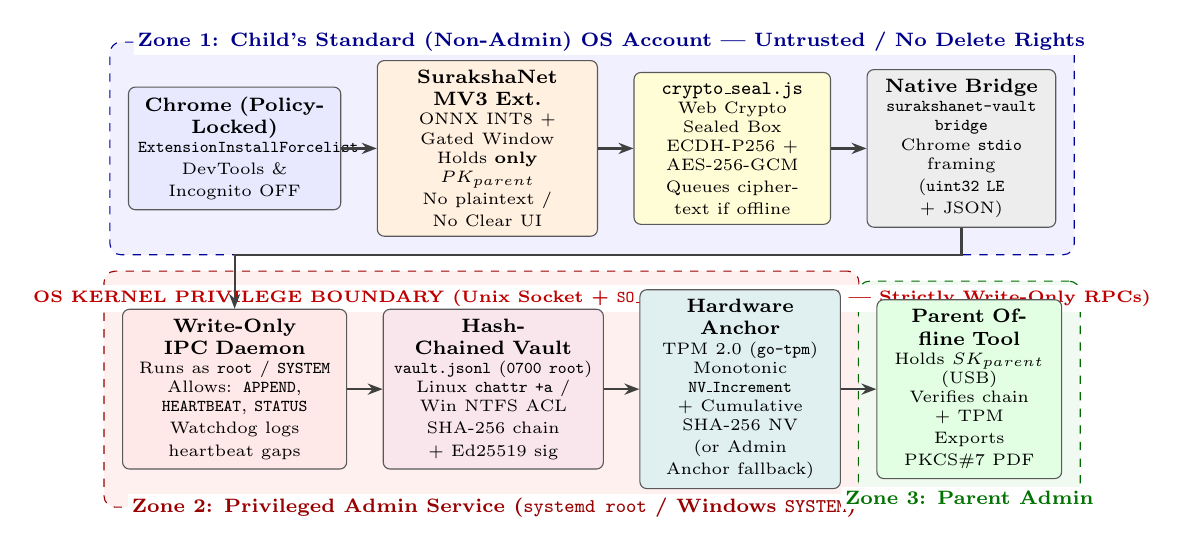
\begin{tikzpicture}[
  box/.style={draw=black!65, rounded corners=2.5pt, fill=#1, align=center,
              font=\fontsize{6.8}{8.0}\selectfont, inner sep=3.5pt},
  zone/.style={draw=#1!60!black, dashed, rounded corners=4pt, fill=#1!6, inner sep=6.5pt},
  arr/.style={-{Stealth[length=1.9mm]}, thick, black!75}
]
  % Zone 1: Child Standard OS Account
  \node[box=blue!9, text width=2.45cm] (chrome) {\textbf{Chrome (Policy-Locked)}\\{\fontsize{5.9}{6.9}\selectfont\texttt{ExtensionInstallForcelist}\\DevTools \& Incognito OFF}};
  \node[box=orange!12, text width=2.55cm, right=4.5mm of chrome] (ext) {\textbf{SurakshaNet MV3 Ext.}\\{\fontsize{5.9}{6.9}\selectfont ONNX INT8 + Gated Window\\Holds \textbf{only} $PK_{\text{parent}}$\\No plaintext / No Clear UI}};
  \node[box=yellow!16, text width=2.25cm, right=4.5mm of ext] (seal) {\textbf{\texttt{crypto\_seal.js}}\\{\fontsize{5.9}{6.9}\selectfont Web Crypto Sealed Box\\ECDH-P256 + AES-256-GCM\\Queues ciphertext if offline}};
  \node[box=gray!14, text width=2.15cm, right=4.5mm of seal] (bridge) {\textbf{Native Bridge}\\{\fontsize{5.9}{6.9}\selectfont\texttt{surakshanet-vault bridge}\\Chrome \texttt{stdio} framing\\(\texttt{uint32 LE} + JSON)}};

  \begin{scope}[on background layer]
    \node[zone=blue, fit=(chrome)(ext)(seal)(bridge),
          label={[fill=white, inner sep=1.5pt, font=\fontsize{6.8}{7.8}\selectfont\bfseries, text=blue!55!black, anchor=west, xshift=3mm]north west:Zone 1: Child's Standard (Non-Admin) OS Account — Untrusted / No Delete Rights}] (z1) {};
  \end{scope}

  % Privilege boundary line
  \coordinate (bL) at ($(z1.south west)+(0,-5.5mm)$);
  \coordinate (bR) at ($(z1.south east)+(0,-5.5mm)$);
  \draw[red!75!black, very thick, densely dashed] (bL) -- (bR)
    node[midway, fill=white, font=\fontsize{6.5}{7.5}\selectfont\bfseries, text=red!75!black, inner sep=2pt]
    {OS KERNEL PRIVILEGE BOUNDARY (Unix Socket + \texttt{SO\_PEERCRED} / Local IPC — Strictly Write-Only RPCs)};

  % Zone 2: Privileged Daemon (root / SYSTEM)
  \node[box=red!9, text width=2.6cm, below=12.5mm of chrome] (ipc) {\textbf{Write-Only IPC Daemon}\\{\fontsize{5.9}{6.9}\selectfont Runs as \texttt{root} / \texttt{SYSTEM}\\Allows: \texttt{APPEND}, \texttt{HEARTBEAT}, \texttt{STATUS}\\Watchdog logs heartbeat gaps}};
  \node[box=purple!10, text width=2.55cm, right=4.5mm of ipc] (chain) {\textbf{Hash-Chained Vault}\\{\fontsize{5.9}{6.9}\selectfont\texttt{vault.jsonl} (\texttt{0700 root})\\Linux \texttt{chattr +a} / Win NTFS ACL\\SHA-256 chain + Ed25519 sig}};
  \node[box=teal!12, text width=2.3cm, right=4.5mm of chain] (tpm) {\textbf{Hardware Anchor}\\{\fontsize{5.9}{6.9}\selectfont TPM 2.0 (\texttt{go-tpm})\\Monotonic \texttt{NV\_Increment}\\+ Cumulative SHA-256 NV\\(or Admin Anchor fallback)}};
  \node[box=green!11, text width=2.1cm, right=4.5mm of tpm] (parent) {\textbf{Parent Offline Tool}\\{\fontsize{5.9}{6.9}\selectfont Holds $SK_{\text{parent}}$ (USB)\\Verifies chain + TPM\\Exports PKCS\#7 PDF}};

  \begin{scope}[on background layer]
    \node[zone=red, fit=(ipc)(chain)(tpm),
          label={[fill=white, inner sep=1.5pt, font=\fontsize{6.8}{7.8}\selectfont\bfseries, text=red!60!black, anchor=west, xshift=3mm]south west:Zone 2: Privileged Admin Service (\texttt{systemd root} / Windows \texttt{SYSTEM})}] (z2) {};
    \node[zone=green!70!black, fit=(parent),
          label={[fill=white, inner sep=1.5pt, font=\fontsize{6.6}{7.6}\selectfont\bfseries, text=green!45!black, anchor=center]south:Zone 3: Parent Admin}] (z3) {};
  \end{scope}

  % Arrows
  \draw[arr] (chrome) -- (ext);
  \draw[arr] (ext) -- (seal);
  \draw[arr] (seal) -- (bridge);
  \draw[arr] (bridge.south) -- ++(0,-3.5mm) -| (ipc.north);
  \draw[arr] (ipc) -- (chain);
  \draw[arr] (chain) -- (tpm);
  \draw[arr] (tpm) -- (parent);
\end{tikzpicture}
}
  \caption{Privilege-separated \textit{SurakshaNet} Parent Evidence Vault architecture. Zone~1 runs inside the child's standard (non-admin) OS account with Chrome locked by machine-wide policies and holding only the parent's public key ($PK_{\text{parent}}$). Zone~2 is a write-only \texttt{root}/\texttt{SYSTEM} Go daemon writing to an admin-only append-only hash chain backed by TPM~2.0 NVRAM. Zone~3 is the offline parent verification and PKCS\#7 signed PDF export workflow holding $SK_{\text{parent}}$.}
  \label{fig:vault_arch}
\end{figure*}

\subsection{Architecture Across the OS Privilege Boundary}
Figure~\ref{fig:vault_arch} illustrates the three-zone architecture implemented in \texttt{vault/} (a single cross-platform Go binary, \texttt{surakshanet-vault}) and \texttt{extension\_v2/}.

\par\textbf{Zone 1: Policy-Locked Chrome Extension (Child's Standard Account).}
During one-time setup, the parent runs an OS-admin installer (\nolinkurl{vault/deploy/linux/install.sh} on Linux or \nolinkurl{install.ps1} on Windows) that writes machine-wide Chrome Enterprise policies \cite{chrome_enterprise_policies} into \nolinkurl{/etc/opt/chrome/policies/managed/surakshanet.json} (Linux) or \texttt{HKLM\textbackslash SOFTWARE\textbackslash\allowbreak Policies\textbackslash Google\textbackslash Chrome} (Windows):
\begin{itemize}
  \item \texttt{ExtensionInstallForcelist} silently installs \textit{SurakshaNet} and removes the user's \textit{Remove} and enable/disable controls.
  \item \texttt{DeveloperToolsAvailability = 2} and \texttt{IncognitoModeAvailability = 1} disable DevTools inspection and unmonitored Incognito bypasses.
  \item \nolinkurl{3rdparty.extensions.<EXT_ID>} injects \texttt{lockMode: true} and \textbf{only} the 65-byte uncompressed P-256 \texttt{parentPublicKey} into read-only \nolinkurl{chrome.storage.managed} (validated by \nolinkurl{managed_schema.json}).
\end{itemize}
When \texttt{lockMode} is active (\nolinkurl{extension_v2/policy.js}, \nolinkurl{store.js}, \nolinkurl{vault_client.js}), \textit{SurakshaNet} \textbf{never writes plaintext messages} to \nolinkurl{chrome.storage.local} (deduplicating via one-way SHA-256 IDs only), disables message-text console logging in \texttt{sw.js}, blocks \texttt{clearIncidents()} and \texttt{exportJSON()}, and switches the popup UI to a locked status panel (Figure~\ref{fig:popup_compare}). If the native daemon is temporarily unreachable, the extension buffers \emph{only} already-encrypted sealed boxes and flushes them on reconnect.

\begin{figure*}[!t]
  \centering
  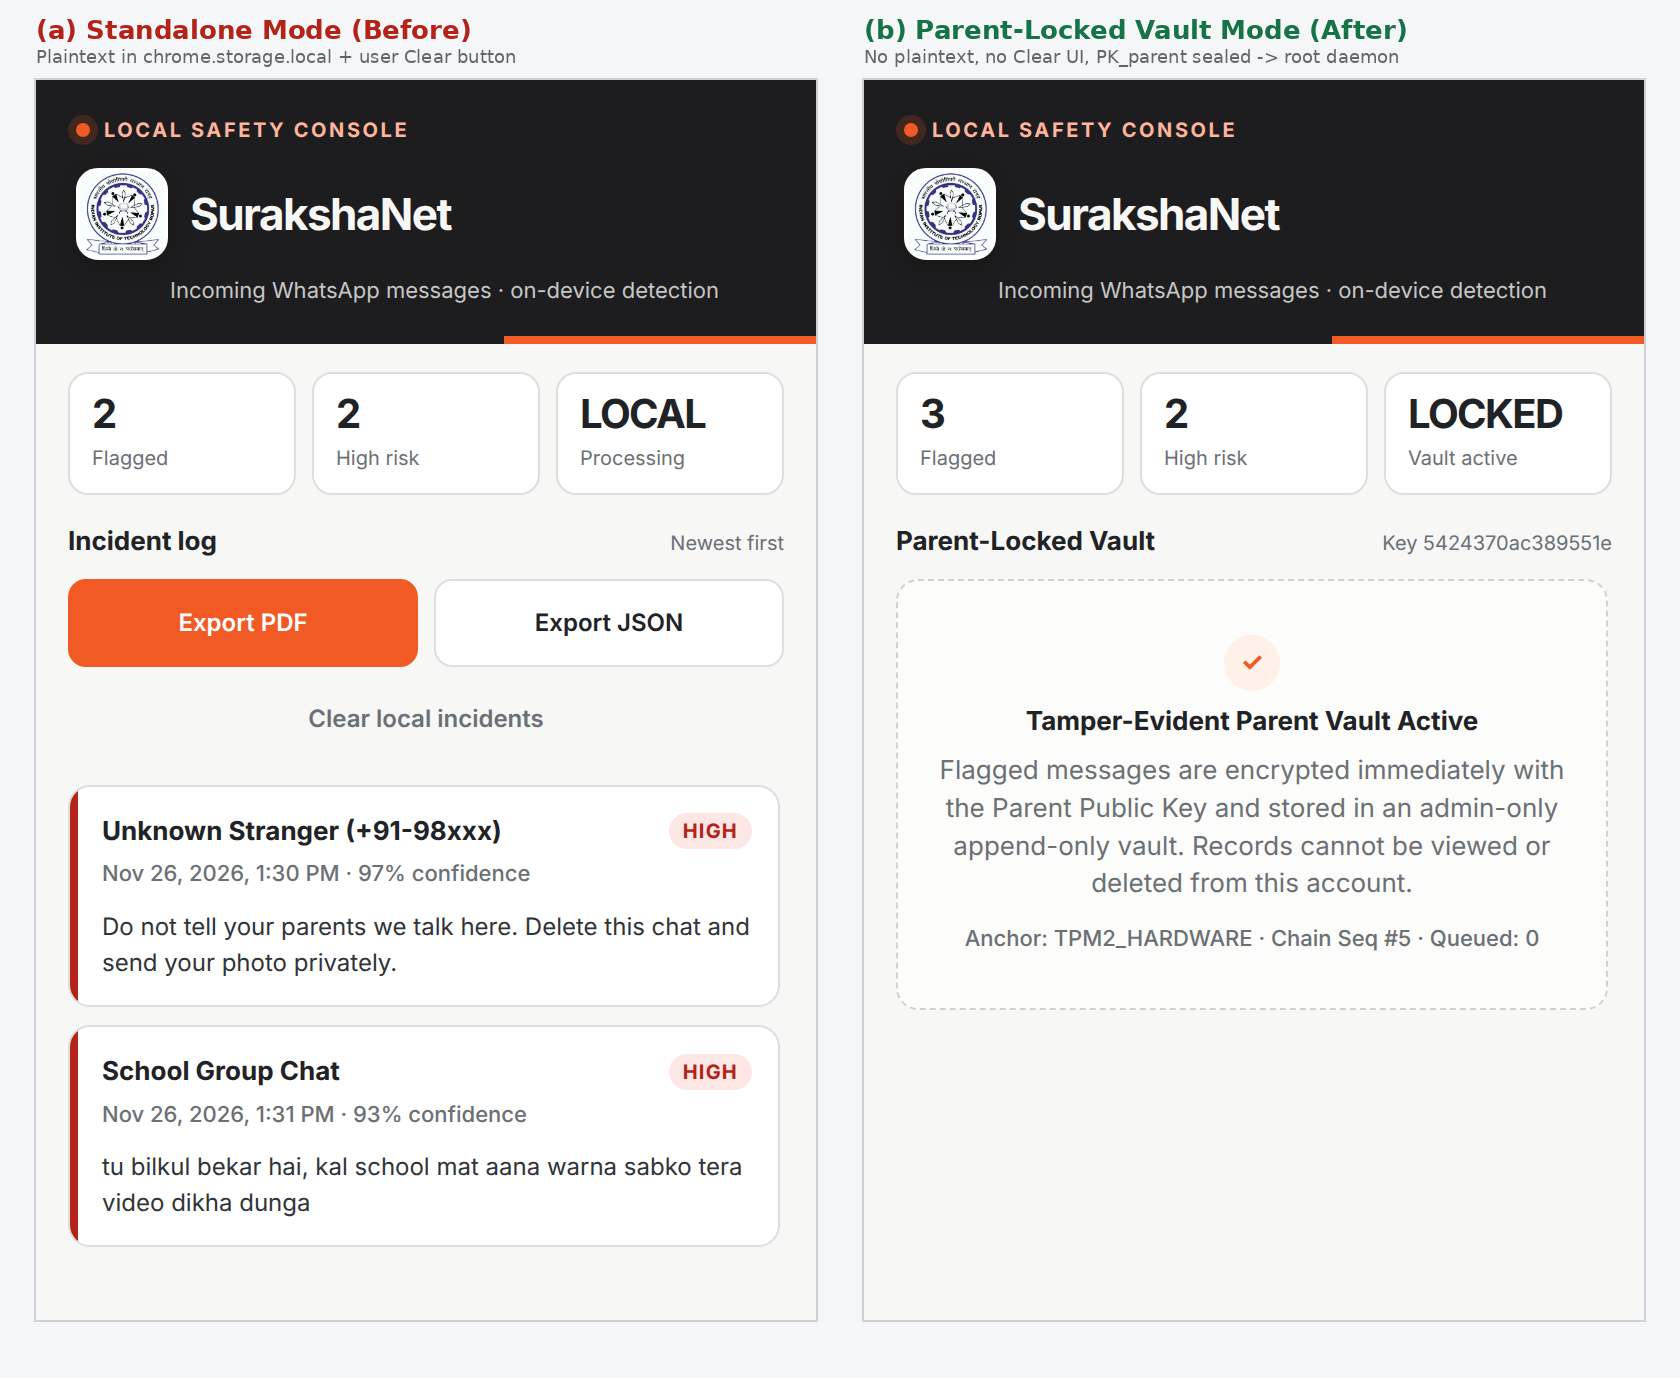
\includegraphics[width=0.96\textwidth]{screenshots/popup_comparison.png}
  \caption{Real Chrome-rendered comparison of \texttt{extension\_v2/popup.html}. Left (a): standalone mode stores plaintext in \texttt{chrome.storage.local} and exposes \textit{Clear local incidents}. Right (b): Parent-Locked Vault mode (activated via \texttt{chrome.storage.managed}) removes all plaintext and delete controls, displays the parent key fingerprint, anchor backend, and chain sequence number, and streams ciphertext to the privileged daemon.}
  \label{fig:popup_compare}
\end{figure*}

\par\textbf{Zone 2: Write-Only Privileged Vault Daemon (\texttt{root} / \texttt{SYSTEM}).}
Because Chrome spawns Native Messaging hosts under the child's OS account, \texttt{surakshanet-vault} \texttt{bridge} acts solely as a stateless \texttt{stdio} relay (\texttt{uint32 LE} length-prefixed JSON) forwarding requests across the OS privilege boundary to an always-on \texttt{surakshanet-vault} \texttt{daemon} running as \texttt{root} (\texttt{systemd}) or \texttt{NT AUTHORITY\textbackslash SYSTEM} (Windows Scheduled Service). Crucially, the local IPC surface (\nolinkurl{vault/internal/ipc/server.go}) is \textbf{strictly write-only}: it exposes only \texttt{APPEND\_INCIDENT}, \texttt{HEARTBEAT}, and \texttt{STATUS}. Any read, list, clear, or delete action is explicitly rejected. On Linux, the daemon extracts kernel-verified caller credentials (\texttt{UID}, \texttt{PID}) via \texttt{SO\_PEERCRED}, opens \texttt{vault.jsonl} exclusively with \texttt{O\_APPEND} + \texttt{fsync} inside a \texttt{0700 root:root} directory, and applies the kernel append-only inode attribute \texttt{FS\_APPEND\_FL} (\texttt{chattr +a}) when supported (Windows enforces equivalent \texttt{SYSTEM} and \texttt{Administrators}-only NTFS ACLs via \texttt{icacls}). A built-in heartbeat watchdog automatically appends a signed \texttt{TAMPER\_HEARTBEAT\_GAP} alert if the extension stops heartbeating (e.g., if a user-level process kills the native bridge).

\subsection{Cryptographic Design and Hardware TPM~2.0 Anchoring}
Figure~\ref{fig:sealedbox_chain} details the end-to-end cryptographic pipeline implemented with byte-for-byte parity between JavaScript Web Crypto (\nolinkurl{extension_v2/crypto_seal.js}, zero external dependencies) and Go (\nolinkurl{vault/internal/crypto/sealedbox.go}).

\begin{figure*}[!t]
  \centering
  \resizebox{\textwidth}{!}{% Cryptographic Sealed-Box + Hash Chain + TPM Anchor pipeline
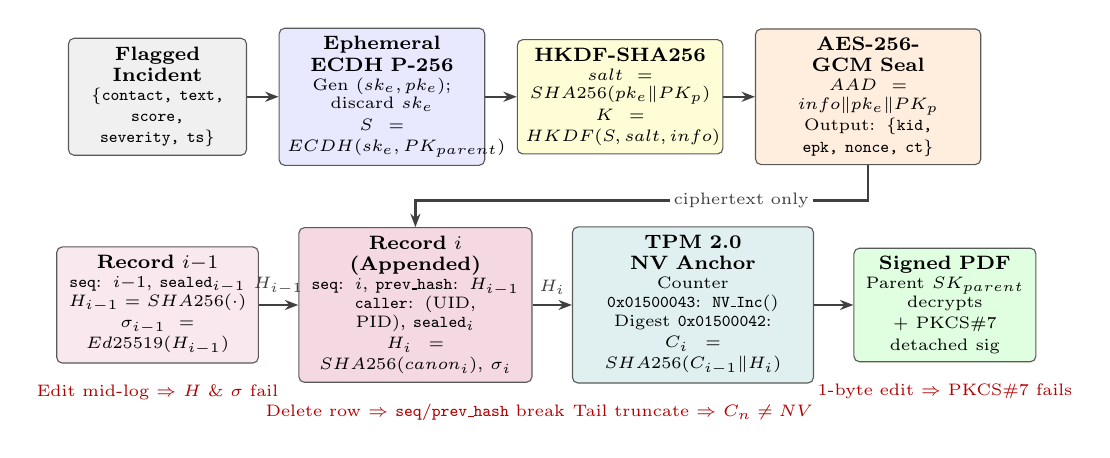
\begin{tikzpicture}[
  cbox/.style={draw=black!65, rounded corners=2pt, fill=#1, align=center,
               font=\fontsize{6.6}{7.7}\selectfont, inner sep=3pt},
  arr/.style={-{Stealth[length=1.7mm]}, thick, black!75}
]
  % Top row: Sealed Box inside Chrome Extension
  \node[cbox=gray!12, text width=2.05cm] (msg) {\textbf{Flagged Incident}\\{\fontsize{5.8}{6.8}\selectfont\texttt{\{contact, text,\\score, severity, ts\}}}};
  \node[cbox=blue!9, text width=2.4cm, right=4mm of msg] (ecdh) {\textbf{Ephemeral ECDH P-256}\\{\fontsize{5.8}{6.8}\selectfont Gen $(sk_e, pk_e)$; discard $sk_e$\\$S = \text{ECDH}(sk_e, PK_{\text{parent}})$}};
  \node[cbox=yellow!16, text width=2.4cm, right=4mm of ecdh] (hkdf) {\textbf{HKDF-SHA256}\\{\fontsize{5.8}{6.8}\selectfont $\text{salt}=\text{SHA256}(pk_e \Vert PK_p)$\\$K = \text{HKDF}(S, \text{salt}, \text{info})$}};
  \node[cbox=orange!13, text width=2.65cm, right=4mm of hkdf] (gcm) {\textbf{AES-256-GCM Seal}\\{\fontsize{5.8}{6.8}\selectfont $\text{AAD} = \text{info}\Vert pk_e \Vert PK_p$\\Output: \texttt{\{kid, epk, nonce, ct\}}}};

  \draw[arr] (msg) -- (ecdh);
  \draw[arr] (ecdh) -- (hkdf);
  \draw[arr] (hkdf) -- (gcm);

  % Bottom row: Hash chain + Ed25519 + TPM NV Extend
  \node[cbox=purple!9, text width=2.35cm, below=11.5mm of msg] (r1) {\textbf{Record $i{-}1$}\\{\fontsize{5.8}{6.8}\selectfont\texttt{seq}: $i{-}1$, \texttt{sealed}$_{i-1}$\\$H_{i-1} = \text{SHA256}(\cdot)$\\$\sigma_{i-1} = \text{Ed25519}(H_{i-1})$}};
  \node[cbox=purple!15, text width=2.75cm, right=5mm of r1] (r2) {\textbf{Record $i$ (Appended)}\\{\fontsize{5.8}{6.8}\selectfont\texttt{seq}: $i$, \texttt{prev\_hash}: $H_{i-1}$\\\texttt{caller}: (UID, PID), \texttt{sealed}$_i$\\$H_i = \text{SHA256}(\text{canon}_i)$, $\sigma_i$}};
  \node[cbox=teal!12, text width=2.85cm, right=5mm of r2] (nv) {\textbf{TPM 2.0 NV Anchor}\\{\fontsize{5.8}{6.8}\selectfont Counter \texttt{0x01500043}: $\texttt{NV\_Inc}()$\\Digest \texttt{0x01500042}:\\$C_i = \text{SHA256}(C_{i-1} \Vert H_i)$}};
  \node[cbox=green!12, text width=2.1cm, right=5mm of nv] (pdf) {\textbf{Signed PDF}\\{\fontsize{5.8}{6.8}\selectfont Parent $SK_{\text{parent}}$ decrypts\\+ PKCS\#7 detached sig}};

  \draw[arr] (r1) -- node[above, font=\fontsize{5.8}{6.8}\selectfont]{$H_{i-1}$} (r2);
  \draw[arr] (gcm.south) -- ++(0,-4.5mm) -| node[pos=0.14, fill=white, inner sep=1.5pt, font=\fontsize{5.8}{6.8}\selectfont]{ciphertext only} (r2.north);
  \draw[arr] (r2) -- node[above, font=\fontsize{5.8}{6.8}\selectfont]{$H_i$} (nv);
  \draw[arr] (nv) -- (pdf);

  % Tamper callouts underneath
  \node[font=\fontsize{5.8}{6.8}\selectfont, text=red!70!black, below=1.5mm of r1] {Edit mid-log $\Rightarrow$ $H$ \& $\sigma$ fail};
  \node[font=\fontsize{5.8}{6.8}\selectfont, text=red!70!black, below=1.5mm of r2] {Delete row $\Rightarrow$ \texttt{seq}/\texttt{prev\_hash} break};
  \node[font=\fontsize{5.8}{6.8}\selectfont, text=red!70!black, below=1.5mm of nv] {Tail truncate $\Rightarrow$ $C_n \neq \text{NV}$};
  \node[font=\fontsize{5.8}{6.8}\selectfont, text=red!70!black, below=1.5mm of pdf] {1-byte edit $\Rightarrow$ PKCS\#7 fails};
\end{tikzpicture}
}
  \caption{Cryptographic evidence pipeline: ephemeral ECDH P-256 + HKDF-SHA256 + AES-256-GCM sealed boxes ensure one-way write confidentiality; SHA-256 hash chaining + daemon Ed25519 signatures + TPM~2.0 NVRAM monotonic counter and cumulative digest detect any edit, mid-log deletion, or tail truncation.}
  \label{fig:sealedbox_chain}
\end{figure*}

\begin{enumerate}
  \item \textbf{One-Way Sealed-Box Encryption.} For every flagged incident, the extension generates a fresh ephemeral ECDH P-256 pair $(sk_e, pk_e)$, computes $S = \text{ECDH}(sk_e, PK_{\text{parent}})$, derives a 256-bit key via HKDF-SHA256 \cite{rfc5869} with salt $\text{SHA-256}(pk_e \Vert PK_{\text{parent}})$, encrypts the canonical JSON payload using AES-256-GCM with $\text{AAD} = \text{info} \Vert pk_e \Vert PK_{\text{parent}}$, and discards $sk_e$. Even the browser extension cannot decrypt a record once sealed. The daemon also rejects any sealed envelope whose \texttt{kid} does not match the configured $PK_{\text{parent}}$.
  \item \textbf{Hash-Chained, Ed25519-Signed Log.} Following the secure audit-log model of Schneier and Kelsey \cite{schneier1999secure}, each record $i$ carries monotonic \texttt{seq}, trusted UTC timestamp, caller \texttt{UID}/\texttt{PID}, \texttt{prev\_hash} $= H_{i-1}$, content digest $H_i = \text{SHA-256}(\text{canonical}_i)$, and signature $\sigma_i = \text{Ed25519}(SK_{\text{daemon}}, H_i)$ using an admin-only daemon key unreadable by standard users.
  \item \textbf{Hardware TPM~2.0 Anchor} (\nolinkurl{vault/internal/tpm/anchor.go})\textbf{.} Hash chains alone cannot detect \emph{tail truncation} (deleting the last $k$ entries). On every append, the daemon extends a cumulative digest $C_i = \text{SHA-256}(C_{i-1} \Vert H_i)$ and commits it to TPM~2.0 hardware \cite{tcg2019tpm2} via \nolinkurl{github.com/google/go-tpm/tpm2} using two persistent NVRAM indices: a hardware-monotonic counter (\texttt{0x01500043}, \texttt{TPMNTCounter}, \texttt{TPM2\_NV\_Increment}) and a 40-byte digest index (\texttt{0x01500042}, \texttt{[seq $\Vert$ $C_i$]}). On machines without an accessible TPM~2.0 device, the vault transparently falls back to an admin-only file anchor (\nolinkurl{ADMIN_FILE_ANCHOR}) and explicitly labels verification output so hardware backing is never overstated.
  \item \textbf{Passphrase-Protected Parent Key \& PKCS\#7 Signed PDFs.} The parent's private keys ($SK_{\text{parent}}$ and ECDSA P-256 PDF signing key) are stored off the child's account in \nolinkurl{parent.key.json}, encrypted via \texttt{scrypt} ($N{=}32768, r{=}8, p{=}1$) + AES-256-GCM. Running \texttt{surakshanet-vault} \texttt{export} verifies the chain and anchor, decrypts all incidents, and generates a PDF~1.4 report embedding a standard ISO~32000-1 \nolinkurl{/adbe.pkcs7.detached} CMS signature \cite{rfc5652} (\nolinkurl{vault/internal/pdf/signed_pdf.go}). Any single-byte edit or trailing byte appended after \texttt{\%\%EOF} immediately invalidates \texttt{surakshanet-vault} \texttt{verify-pdf}.
\end{enumerate}

\subsection{Zero-Login Operational User Flow}
No cloud account or user login is required. Figure~\ref{fig:user_flow} summarises the three-phase lifecycle: (1)~the parent runs the admin installer once ($\sim$2\,minutes), moves \texttt{parent.key.json} to a USB drive or personal device, and leaves the child on a standard OS account; (2)~the child browses normally with zero login while incidents are sealed and anchored silently; (3)~when needed, the parent runs \texttt{verify} and \texttt{export} offline to obtain a cryptographically verified, digitally signed PDF report.

\begin{figure*}[!t]
  \centering
  \resizebox{\textwidth}{!}{% Three-phase zero-login user operational workflow
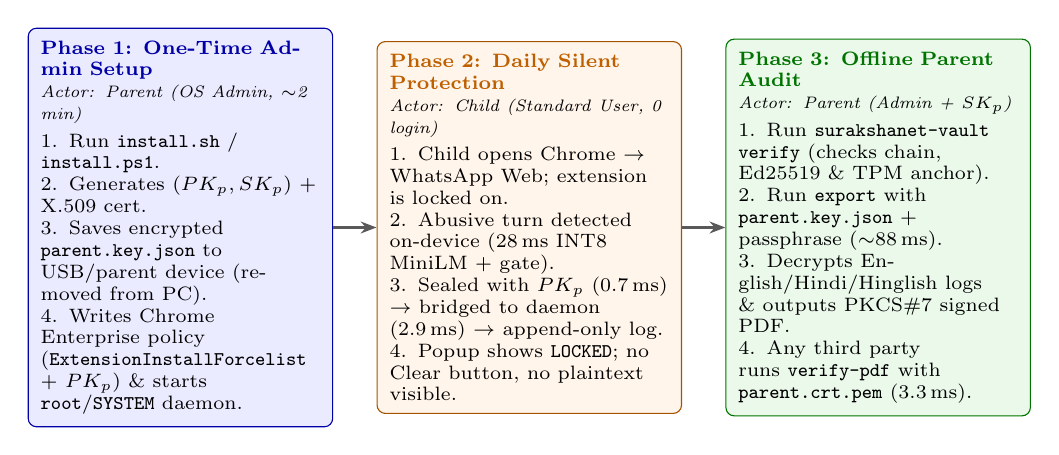
\begin{tikzpicture}[
  phase/.style={draw=#1!65!black, rounded corners=3pt, fill=#1!8, align=left,
                font=\fontsize{6.6}{7.9}\selectfont, inner sep=4.5pt, text width=3.55cm},
  arr/.style={-{Stealth[length=2mm]}, very thick, black!65}
]
  \node[phase=blue] (p1) {
    \textbf{\textcolor{blue!65!black}{Phase 1: One-Time Admin Setup}}\\
    {\fontsize{5.9}{7}\selectfont\textit{Actor: Parent (OS Admin, $\sim$2 min)}}\\[2pt]
    1. Run \texttt{install.sh} / \texttt{install.ps1}.\\
    2. Generates $(PK_p, SK_p)$ + X.509 cert.\\
    3. Saves encrypted \texttt{parent.key.json} to USB/parent device (removed from PC).\\
    4. Writes Chrome Enterprise policy (\texttt{ExtensionInstallForcelist} + $PK_p$) \& starts \texttt{root}/\texttt{SYSTEM} daemon.
  };

  \node[phase=orange, right=5.5mm of p1] (p2) {
    \textbf{\textcolor{orange!75!black}{Phase 2: Daily Silent Protection}}\\
    {\fontsize{5.9}{7}\selectfont\textit{Actor: Child (Standard User, 0 login)}}\\[2pt]
    1. Child opens Chrome $\rightarrow$ WhatsApp Web; extension is locked on.\\
    2. Abusive turn detected on-device (28\,ms INT8 MiniLM + gate).\\
    3. Sealed with $PK_p$ (0.7\,ms) $\rightarrow$ bridged to daemon (2.9\,ms) $\rightarrow$ append-only log.\\
    4. Popup shows \texttt{LOCKED}; no Clear button, no plaintext visible.
  };

  \node[phase=green!70!black, right=5.5mm of p2] (p3) {
    \textbf{\textcolor{green!45!black}{Phase 3: Offline Parent Audit}}\\
    {\fontsize{5.9}{7}\selectfont\textit{Actor: Parent (Admin + $SK_p$)}}\\[2pt]
    1. Run \texttt{surakshanet-vault verify} (checks chain, Ed25519 \& TPM anchor).\\
    2. Run \texttt{export} with \texttt{parent.key.json} + passphrase ($\sim$88\,ms).\\
    3. Decrypts English/Hindi/Hinglish logs \& outputs PKCS\#7 signed PDF.\\
    4. Any third party runs \texttt{verify-pdf} with \texttt{parent.crt.pem} (3.3\,ms).
  };

  \draw[arr] (p1) -- (p2);
  \draw[arr] (p2) -- (p3);
\end{tikzpicture}
}
  \caption{Zero-login three-phase operational flow separating OS Administrator setup and offline private-key auditing from the child's daily Standard User session.}
  \label{fig:user_flow}
\end{figure*}

\subsection{Security Evaluation, Live Tamper Proofs, and Latency}
Table~\ref{tab:threat_matrix} contrasts the attack surface before and after introducing the vault. We validated all guarantees using Go race-detector unit tests (\texttt{go test -race ./...} across \texttt{crypto}, \texttt{chain}, \texttt{ipc}, and \texttt{pdf}) and a cross-language end-to-end suite (\texttt{vault/e2e\_test.mjs}) sealing English, Devanagari Hindi, and Hinglish messages in JavaScript Web Crypto, streaming them through \texttt{surakshanet-vault bridge} to \texttt{daemon}, verifying exact UTF-8 decryption parity, exporting a signed PDF, and executing live attacks.

\begin{table*}[t]
\centering
\caption{Security comparison before (\texttt{extension\_v2} local storage) and after adding the Admin-Locked Parent Evidence Vault.}
\label{tab:threat_matrix}
\small
\begin{tabularx}{\textwidth}{@{}l X X X@{}}
\toprule
\textbf{Threat / Attack Vector} & \textbf{Before (\texttt{chrome.storage.local})} & \textbf{After (Parent-Locked Vault)} & \textbf{Enforcement Mechanism} \\
\midrule
Remove or disable extension & One click in \nolinkurl{chrome://extensions} & \textbf{Blocked} for Standard OS user & Chrome \texttt{ExtensionInstallForcelist} in \texttt{HKLM} / \nolinkurl{/etc/opt/chrome/policies/managed} \\
Click \textit{Clear} / wipe storage & All evidence permanently lost & \textbf{Blocked / No plaintext in browser} & Managed \texttt{lockMode} hides Clear UI; \texttt{store.js} writes ciphertext to daemon only \\
Read saved chats on disk & Plaintext JSON readable by user & \textbf{Unreadable} (OS + crypto) & \texttt{0700 root}/NTFS ACL + ECDH-P256 sealed box ($SK_{\text{parent}}$ offline) \\
Send wipe RPC over IPC & N/A & \textbf{Rejected} (Figure~\ref{fig:tamper_term}) & Strictly write-only IPC (\texttt{APPEND}, \texttt{HEARTBEAT}, \texttt{STATUS} only) \\
Edit or delete middle record & Undetectable & \textbf{Immediately caught} & Broken SHA-256 \texttt{prev\_hash}, sequence gap, invalid Ed25519 sig \\
Truncate tail of \texttt{vault.jsonl} & Undetectable & \textbf{Immediately caught} (Figure~\ref{fig:tamper_term}) & Cumulative digest $C_n$ \& count mismatch against TPM~2.0 / Admin Anchor \\
Kill bridge / detach extension & Silent monitoring failure & \textbf{Logged as tamper alert} & Daemon heartbeat watchdog records \texttt{TAMPER\_HEARTBEAT\_GAP} \\
Modify 1 byte of exported PDF & Unsigned \texttt{jsPDF}, trivial to fake & \textbf{Immediately caught} (Figure~\ref{fig:tamper_term}) & ISO 32000-1 \texttt{/adbe.pkcs7.detached} signature + full-file \texttt{/ByteRange} \\
\bottomrule
\end{tabularx}
\end{table*}

Figures~\ref{fig:e2e_term}, \ref{fig:tamper_term}, and \ref{fig:signed_pdf_shot} show real captured outputs from our end-to-end verification, simulated attack suite, and generated PKCS\#7 signed PDF.

\begin{figure*}[!t]
  \centering
  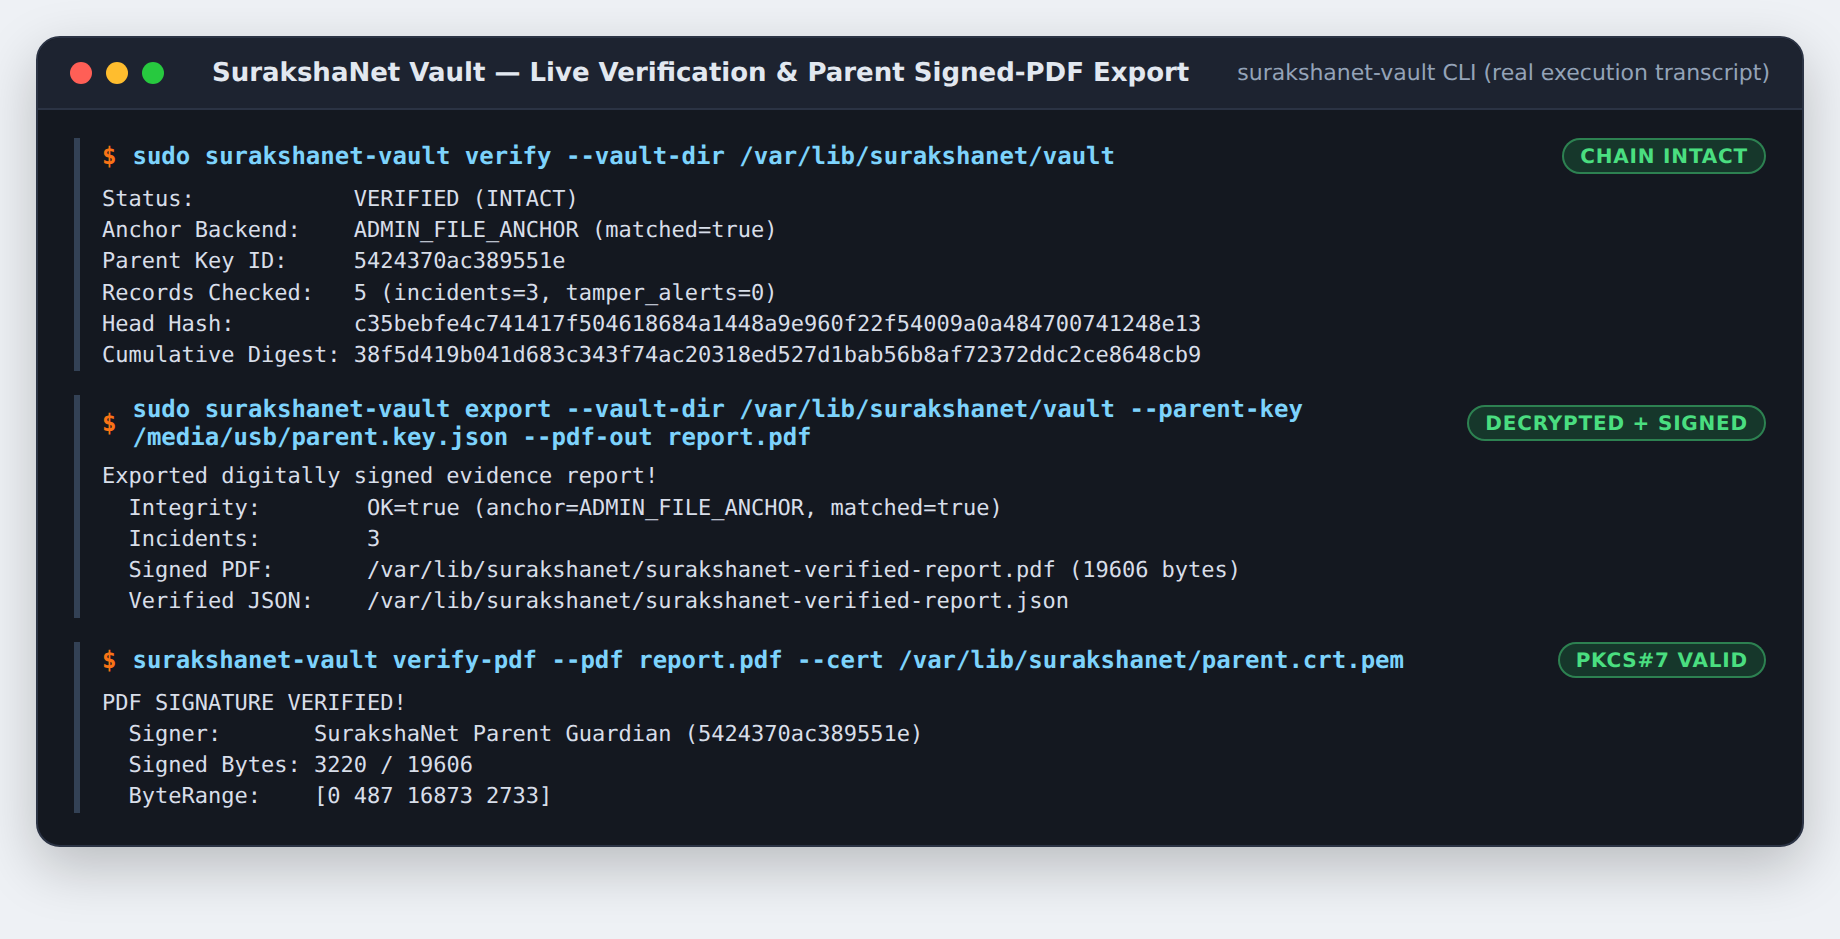
\includegraphics[width=0.92\textwidth]{screenshots/terminal_e2e_verify.png}
  \caption{Live CLI verification (\texttt{verify}), parent decryption + PKCS\#7 PDF export (\texttt{export}), and cryptographic PDF signature check (\texttt{verify-pdf}) captured directly from \nolinkurl{surakshanet-vault}.}
  \label{fig:e2e_term}
\end{figure*}

\begin{figure*}[!t]
  \centering
  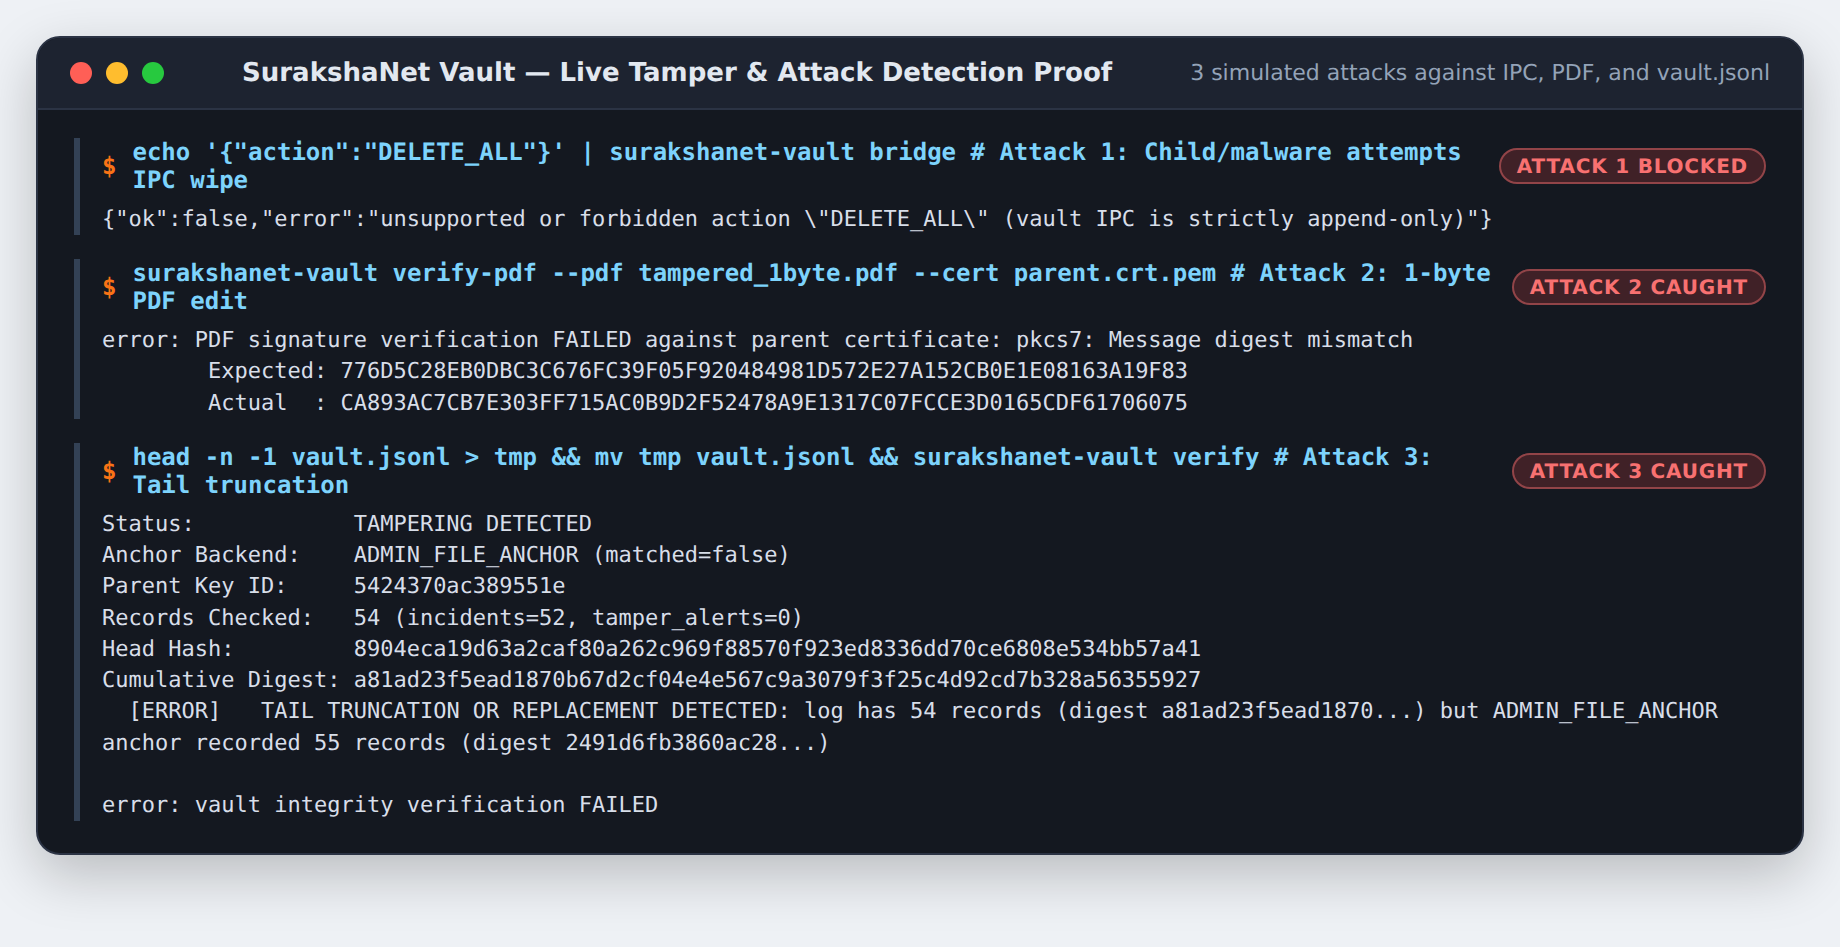
\includegraphics[width=0.92\textwidth]{screenshots/terminal_tamper_attacks.png}
  \caption{Live attack proofs: (1)~IPC \texttt{DELETE\_ALL} rejected as forbidden on the write-only socket, (2)~1-byte PDF edit caught via PKCS\#7 digest mismatch, and (3)~tail truncation of \texttt{vault.jsonl} caught via anchor count and cumulative digest mismatch.}
  \label{fig:tamper_term}
\end{figure*}

\begin{figure}[!t]
  \centering
  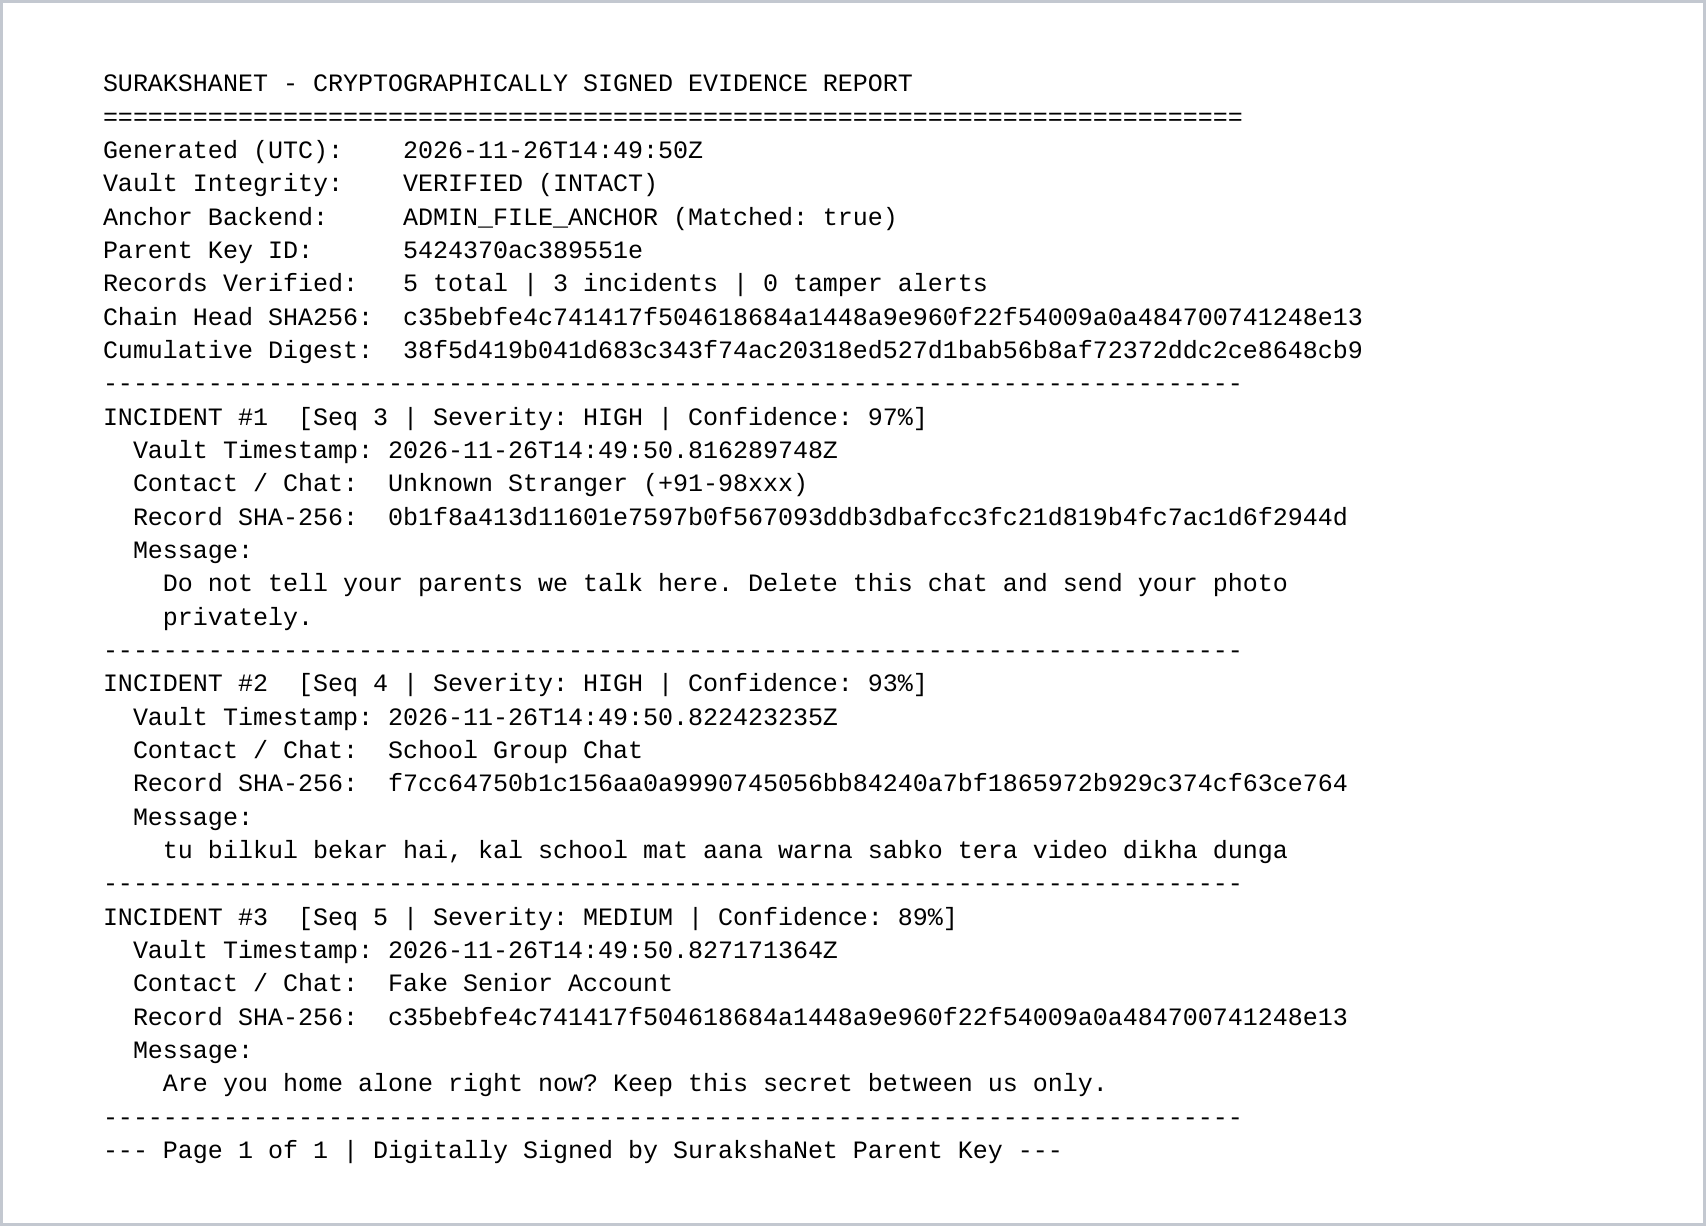
\includegraphics[width=\columnwidth]{screenshots/signed_pdf_preview.png}
  \caption{Rendered page of a real PKCS\#7 digitally signed PDF exported by \texttt{surakshanet-vault} \texttt{export}, embedding chain integrity metadata, per-incident SHA-256 hashes, and decrypted multilingual evidence.}
  \label{fig:signed_pdf_shot}
\end{figure}

\begin{figure}[!t]
  \centering
  \resizebox{\columnwidth}{!}{% Real measured vault latency microbenchmark (vault/bench_report.json)
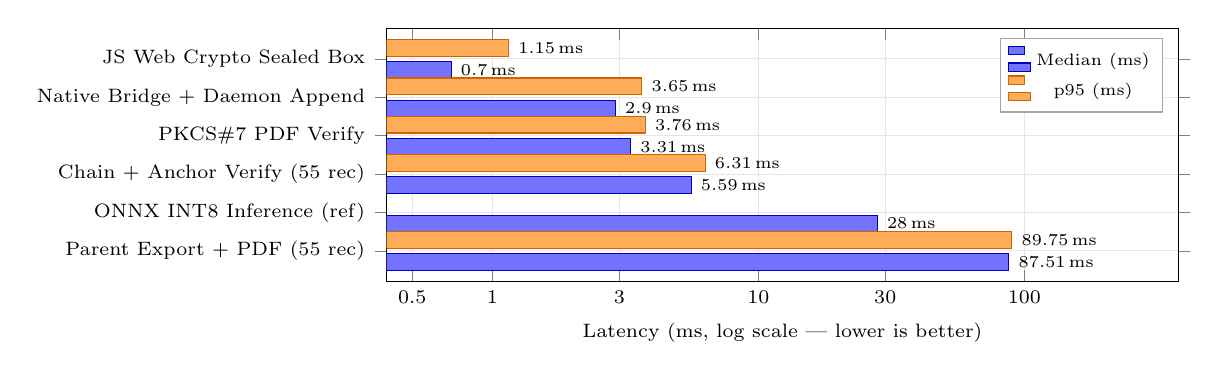
\begin{tikzpicture}
\begin{axis}[
  xbar,
  width=0.96\columnwidth,
  height=4.8cm,
  bar width=6pt,
  enlarge y limits=0.16,
  xlabel={Latency (ms, log scale — lower is better)},
  xlabel style={font=\fontsize{7}{8}\selectfont},
  xmode=log,
  log origin=infty,
  xmin=0.4, xmax=380,
  xtick={0.5, 1, 3, 10, 30, 100},
  xticklabels={0.5, 1, 3, 10, 30, 100},
  tick label style={font=\fontsize{6.6}{7.6}\selectfont},
  symbolic y coords={
    {Parent Export + PDF (55 rec)},
    {ONNX INT8 Inference (ref)},
    {Chain + Anchor Verify (55 rec)},
    {PKCS\#7 PDF Verify},
    {Native Bridge + Daemon Append},
    {JS Web Crypto Sealed Box}
  },
  ytick=data,
  point meta=rawx,
  nodes near coords={\pgfmathprintnumber[fixed,precision=2]{\pgfplotspointmeta}\,ms},
  nodes near coords style={font=\fontsize{5.9}{6.8}\selectfont, anchor=west},
  legend style={at={(0.98,0.96)}, anchor=north east, font=\fontsize{6.2}{7.2}\selectfont,
                draw=black!35, fill=white, inner sep=2.5pt},
  grid=major,
  major grid style={gray!20},
]
  \addplot[fill=blue!55, draw=blue!75!black] coordinates {
    (0.70,{JS Web Crypto Sealed Box})
    (2.90,{Native Bridge + Daemon Append})
    (3.31,{PKCS\#7 PDF Verify})
    (5.59,{Chain + Anchor Verify (55 rec)})
    (28.00,{ONNX INT8 Inference (ref)})
    (87.51,{Parent Export + PDF (55 rec)})
  };
  \addplot[fill=orange!65, draw=orange!80!black] coordinates {
    (1.15,{JS Web Crypto Sealed Box})
    (3.65,{Native Bridge + Daemon Append})
    (3.76,{PKCS\#7 PDF Verify})
    (6.31,{Chain + Anchor Verify (55 rec)})
    (89.75,{Parent Export + PDF (55 rec)})
  };
  \legend{Median (ms), p95 (ms)}
\end{axis}
\end{tikzpicture}
}
  \caption{Measured latency of vault operations on Linux \texttt{x86\_64} (\nolinkurl{vault/bench_report.json}, $n{=}53$ appends and $n{=}10$ full-vault runs on 55 records) versus the 28\,ms ONNX inference baseline.}
  \label{fig:vault_bench}
\end{figure}

\par\textbf{Performance Overhead.} Figure~\ref{fig:vault_bench} reports real microbenchmark measurements (\nolinkurl{vault/bench_vault.mjs}, saved in \nolinkurl{vault/bench_report.json}). Web Crypto sealed-box encryption takes a median of \textbf{0.70\,ms} (p95 1.15\,ms), and the full Native Messaging bridge + daemon \texttt{O\_APPEND} + \texttt{fsync} + Ed25519 + anchor round-trip takes \textbf{2.90\,ms} (p95 3.65\,ms). Thus, end-to-end tamper-evident capture adds only \textbf{3.60\,ms} on top of the 28\,ms ONNX inference latency, and runs solely when a message is flagged. Offline verification of 55 chained records takes \textbf{5.59\,ms}, PDF signature verification takes \textbf{3.31\,ms}, and full parent export (intentionally dominated by \texttt{scrypt} passphrase key derivation) completes in \textbf{87.51\,ms}. The Go binary cross-compiles cleanly to Linux (\texttt{amd64}), Windows (\texttt{amd64}), and macOS (\texttt{arm64}).

%==============================================================
\section{Final Deployed Configuration}
Based on the complete evaluation, the current \textit{SurakshaNet} deployment combines the \textbf{INT8 MiniLM encoder with the gated conversational window} and the \textbf{Parent-Locked Tamper-Evident Vault}, achieving:
\begin{itemize}
    \item \textbf{84.2\%} accuracy on single-message classification,
    \item \textbf{76.1\%} recall on split-narrative conversations,
    \item \textbf{82.9\%} accuracy when abusive content appears after small talk,
    \item \textbf{83.0\%} accuracy on benign conversations, and
    \item \textbf{3.60\,ms} median end-to-end vault sealing and privileged append overhead with 100\% detection of IPC wipe attempts, mid-log edits/deletions, tail truncation, and 1-byte PDF tampering.
\end{itemize}
The deployed extension does not send user conversations to Amazon Bedrock or any other cloud-based LLM; the Bedrock experiments were conducted solely for benchmarking, and both inference and evidence preservation remain completely local, preserving the privacy-first design. The five-class thread models are research artifacts; the extension itself still uses the binary model.

\subsection*{Limitations and next steps}
The five-class data are generated by an LLM and checked by automatic rules; no human annotators reviewed them, so the scores in Section~\ref{sec:models} describe the synthetic distribution. A first zero-shot check of the synthetic-trained models on real conversation data (CAD, ConvAbuse, PRISM) gave AUROC between 0.47 and 0.74, so we see the dataset today as a controlled benchmark and as training material to be mixed with real data. Our Hinglish text is machine-converted and less code-mixed than human Hinglish, the cloud-LLM comparison uses small subsets, and latency of the five-class models was measured natively rather than in the browser. For the evidence vault (Section~\ref{sec:vault}), three honest trust boundaries remain: (1)~no purely local vault can survive a full physical hard-drive wipe or a compromised OS Administrator/\texttt{root} account—defending against full disk destruction requires an optional zero-knowledge remote mirror of the already-encrypted sealed boxes (e.g., S3 Object Lock or a companion parent app); (2)~on non-domain-joined consumer Windows and macOS devices, Chrome restricts \texttt{ExtensionInstallForcelist} to Chrome Web Store extensions (requiring an unlisted store listing or Chrome Browser Cloud Management); and (3)~local capture proves post-capture integrity rather than WhatsApp server provenance (which would require network-level TLS attestation). Next steps are adding real threaded data with held-out evaluation, integrating the five-class INT8 thread model into the extension, testing hardware TPM~2.0 NV anchoring across consumer laptops, and adding optional zero-knowledge encrypted sync plus RFC~3161/OpenTimestamps anchoring.

%==============================================================
\section{Conclusion}
\textit{SurakshaNet} demonstrates that proactive, multilingual moderation and forensic-grade child safety are technically viable entirely on the edge. By combining low-latency local INT8 inference, gated conversational-context handling, and an OS-admin-locked, cryptographically verifiable \textit{Parent Evidence Vault} (Web Crypto sealed boxes, a write-only \texttt{root}/\texttt{SYSTEM} append-only daemon, TPM~2.0 anchoring, and PKCS\#7 signed PDFs), the system closes the critical tampering gap of browser-only extensions while adding only 3.6\,ms of capture latency and zero cloud plaintext exposure. Alongside the 105{,}000-thread five-class benchmark (97.9\% synthetic test accuracy at 118\,MB INT8), this provides an end-to-end foundation for trustworthy, privacy-first protection of children and women online.

\bibliographystyle{ACM-Reference-Format}
\bibliography{references}

\end{document}
